
%%%%% Document Setup %%%%%%%%

\documentclass[12pt,onecolumn]{revtex4-2}    % Font size (10,11 or 12pt) and column number (one or two).


\usepackage{times}                          % Times New Roman font type
\usepackage{float}
\usepackage{booktabs}
\usepackage{amsfonts}
\usepackage{subcaption}

\usepackage[a4paper, left=2.5cm, right=2.5cm,top=2.5cm, bottom=2.5cm]{geometry}       % Defines paper size and margin length, 1.85 for all
\renewcommand{\baselinestretch}{1}

\usepackage[font=small, labelfont=bf]{caption}                      % Defines caption font size as 9pt and caption title bolded


\usepackage{graphics,graphicx,epsfig,ulem}	% Makes sure all graphics works
\usepackage{amsmath} 						% Adds mathematical features for equations

\usepackage{etoolbox}                       % Customise date to preferred format
\captionsetup{justification=raggedright,singlelinecheck=false}

\makeatletter
\patchcmd{\frontmatter@RRAP@format}{(}{}{}{}
\patchcmd{\frontmatter@RRAP@format}{)}{}{}{}
\renewcommand\Dated@name{}
\makeatother

\usepackage{fancyhdr}


\pagestyle{fancy}                           % Insert header
\fancyhead{} % clear all header fields
\fancyhead[L]{\fontsize{10}{12} \selectfont Rebecca J. Hedley}
\fancyhead[R]{\fontsize{10}{12}
\selectfont Replicating Mars' Climate: Applying a 1-Dimensional Energy Balance Climate Model}

%\renewcommand{\headrulewidth}{0pt}
%\lhead{Rebecca J. Hedley}                          % Your name
%\rhead{Replicating Mars' Climate: Applying a 1-Dimensional Energy Balance Climate Model}            % Your report title               

\def\bibsection{\section*{References}}        % Position reference section correctly
\bibliographystyle{plain}

%%%%% Document %%%%%    
\begin{document}


\title{Replicating Mars' Climate: Applying a One-Dimensional Energy Balance Climate Model} 
\date{Submitted: \today{}}
\author{Rebecca J. Hedley}
\affiliation{\normalfont Level 4 Project, MPhys Physics\\ Supervisor: Drs. Richard Wilman and Craig Testrow\\ Department of Physics, Durham University}


\begin{abstract}              

A one-dimensional energy balance model (EBM) is built using the finite difference method, based on a differential equation encompassing the effects of heat capacity, solar insolation, albedo, meridional heat diffusion, and outgoing radiation. Mean annual temperature values agree to a latitudinally averaged value of 1\% to Earth climate fit from literature, and to within 3.2\% when the same model is applied to Mars. Seasonal variations are clearly observed in the model and replicate more extreme variations expected on Mars, as well as the combined effects of obliquity and an eccentric orbit. Further work involving CO2 cycle modelling is discussed to improve the Mars model given the importance of the annual pressure cycle.

\end{abstract}

\maketitle

\thispagestyle{plain} % produces page number for front page

\tableofcontents

\section{Introduction} 

\subsection{Motivation}

Mars' current climate is cold and dry, and its atmospheric volume is less than 1\% of Earths. Despite this, there exists evidence for an active hydrological cycle in its past. Branching tributaries beginning near geographic peaks indicate precipitation, and the large valley networks these create are expected to have formed over timescales of $10^{5}$ - $10^{7}$ years. \cite{W16} %more evidence for water

It is unlikely that Ancient Mars' wet climate was similar to that of Earths. Constraints on luminosity, orbit, and radiative transfer disfavour a warmer climate, suggesting that the water cycle was limited in volume and intermittent during the ancient Noachian period (between 3 and 3.5Ga ago). Geophysical evidence supports this, given that the lack of consistent glaciation similarly points towards a small water inventory. %more evidence for episodic melting

With climate studies, we can make preliminary insights into whether Mars could have, or can in the future, host life. %motivations for understanding earths climate and astrobiology

\subsection{Climate Modelling}

\subsubsection{Energy Balance Models}
%"habitable climates" has some good info
Energy balance models predict global temperatures by a radiative energy budget, estimating energy received from the Sun and energy retained or reflected by the planet. The most simple EBM is the zero-dimensional case, a model which predicts a single mean surface temperature to the whole planet by assuming that the energy received is equal to the energy lost in a steady state solution. The 0D EBM neglects varying land distributions (and therefore temperature-dependent heat capacities, albedo values, and outgoing radiation) and heat diffusion between latitudes. They can provide relatively accurate estimates for global mean temperature \cite{L20}, however they cannot provide temperature as a function of latitude, and so are not appropriate for this study of Mars' climate.
\

One-dimensional EBMs, such as the model used in this study, split the planet into latitude bands and assess the temperature of each based on local variables such as solar insolation and ice distribution. 1D EBMs most importantly allow for meridional heat transport, an important factor in the local latitudinal energy budget for planets with a thick enough atmosphere \cite{SMS08}, and therefore important for the Earth validation study and later, a study of Mars' pressure variations. As a result of the inclusion of heat diffusion, it is possible that each region at any particular time will not satisfy the energy budget condition of energy in = energy out. This is also possible for the planet as a whole on any day, especially due to an eccentric orbit. Deviations from the energy budget are what create 

\subsubsection{General Circulation Models}

General circulation models (GCMs) are more complex three- (or four-) dimensional climate models which are based on fluid equations. Earth is split into horizontal grid cells longitudinally and latitudinally, and also split vertically based on height from surface or pressure. Systems which apply on scales smaller than that of the resolution of the grid, such as ice-albedo feedback or cloud effects on radiative flux, are parametrised, and these parametrisations create the largest source of error within a GCM \cite{CBZH}. Despite this, GCMs remain the most accurate computational representations of climate.
\

GCMs have had success modelling the CO2 cycle on Mars. Unlike EBMs, which assume CO2 condenses directly on the surface, GCMs allow for CO2 condensing in the atmosphere. Atmospheric CO2 behaves much differently to ice cap CO2 in that, whereas ice deposits are effectively transparent at infrared wavelengths, atmospheric CO2 particles efficiently scatter heat and therefore contribute to global cooling. Such effects on Mars have been observed to decrease total polar condensation rates by 10 - 20\% during the winter \cite{FP96}, therefore also affecting ice-albedo feedback and decreasing heat diffusion due to a reduced atmosphere. 
 
\section{Theory and Methods} 
\subsection{Energy Budget}

The infrared radiation received and retained by the atmosphere is dependent on the total solar flux $S$ received at each band, and the albedo $A$ of that band,
\begin{center}
$I(T) = S(1-A(T))$.
\end{center}
\subsubsection{Incoming Flux}

Total solar flux in each latitude band is proportional to the cosine of solar zenith angle $z$, which is expressed  as a function of latitude $\theta$, solar hour angle $h$, and solar declination $\delta$:

\begin{center}
$\cos z = \sin \theta \sin \delta + \cos \theta \cos \delta \cos h.$
\end{center}

The declination angle is a sinusoidal function dependent on orbital longitude and obliquity $\delta_{0}$, which reaches its extrema at the solstices. Solar hour angle describes the angular displacement of the Sun in a planets sky from the meridian, and is zero degrees at noon. 
\
In order to find a diurnally averaged value for incoming solar flux, the cosine of solar zenith angle $z$ must be averaged over one rotation. First it is averaged over solar hour angle $h$ = - $H$ to + $H$, with H as radian half-day length,

\begin{center}
$\cos H = -\tan \theta \tan \delta$,
\end{center}

which corresponds to the fraction of a day during which the sun is above the horizon. 
\begin{center}
$\overline{\cos z}$ = $\frac{\int_{-H}^{H} \sin\theta \sin\delta + \cos\theta \cos\delta \cosh dh}{\int_{-H}^{H} dh}$

$= \sin\theta \sin \delta + \cos\theta \cos\delta \frac{\sin H}{H}$.
\end{center}

If, during summers at the poles for example, the sun remains above the horizon for a complete day then $H$ = $\pi$ according to the above definition. At latitudes where the Sun remains in the sky for a fraction of a rotation, the average $\overline{\cos z}$ must be scaled then by $\frac{H}{\pi}$. In order to generalise to any planet with semimajor axis $a$ in AU, (X) is also scaled by a $\frac{1}{a^{2}}$ term. Multiplying by these factors and also by solar constant $q$, we find diurnally averaged incident solar flux $S_{0}$,

\begin{center}
$S_{0} = \frac{q}{\pi}(\frac{1.0 AU}{a})^{2}(H\sin \theta \sin \delta + \cos \theta \cos \delta \sin H)$.
\end{center}

As of yet, we have assumed a circular orbit.
Total insolation received by a planet at a given time is a function of the position in its orbit (given that the orbit is not perfectly circular), and the solar zenith angle at each latitude. The instantaneous Sun-planet distance is given by the following expression,

\begin{center}
$r$ = $\frac{a(1-e^{2})}{1 + e \cos \theta}$
\end{center}

where $e$ is the eccentricity of the orbit, $a$ is its semimajor axis, and $\theta$ is the true anomaly, an angular quantity which defines the position of a body in its orbit in respect to its periapsis. From the instantaneous position $r$ we can then include the effect of eccentricity on daily insolation by invoking the inverse square law,

\begin{center}
$S_{eccentric} = \frac{S_{0}}{r^{2}},$
\end{center}

where $S_{0}$ is the original expression (X) derived for a body with zero orbital eccentricity.

\subsubsection{Outgoing Flux}
Three prescriptions were tested for infrared cooling and albedo functions. The first two assume that the planet is a blackbody and therefore radiates energy proportional to $T^{4}$, which is then reduced through an optically thick atmosphere which reradiates heat back to the planet. The two models differ in that the second has a temperature dependent optical thickness, $\tau_{IR}(T)$, which acts to decrease infrared radiation escaping the atmosphere as the surface temperature increases. This reflects the temperature-dependent greenhouse effect, in which heat retention scales with the amount of water vapour in the atmosphere due to absorption. The third model is a simple linear relation obtained by applying a least squares fit to outgoing infrared flux data from satellite observations. The $\tau_{IR}$ models are borrowed from SMS08 \cite{SMS08}, and the linear model is borrowed from NC79 \cite{NC79}. These are outlined in Table I. 
\\
\begin{table}
\begin{tabular}{ccc} \toprule
    Model & IR Cooling Function & Albedo Function \\ \midrule
    1  & $I(T) = \frac{\sigma T^{4}}{1+ \frac{3}{4}\tau_{IR}^{0}}$ & $A(T) = 0.5 - 0.2 \tanh \frac{T - 268}{5}$ \\
    2  & $I(T) = \frac{\sigma T^{4}}{1+ \frac{3}{4}\tau_{IR}(T)}$  & $A(T) = 0.525 - 0.245 \tanh \frac{T - 268}{5}$ \\
    3  & $I(T) = A + BT $  & $A(T) = 0.475 - 0.225 \tanh \frac{T - 268}{5}$ \\
\bottomrule
\end{tabular}
\caption{Model 1 has fixed optical thickness $\tau_{IR}^{0}$ = 1. Model 2 has temperature dependent optical thickness $\tau_{IR}(T) = \frac{0.79}{(T/273)^{3}}$. Model 3 has constants A = 2.033 $\times 10^{2} Jm^{-2}s^{-1}$, B = 2.094 $J m^{-2} s^{-1} K^{-1}$}.
\end{table}

Albedo is dependent on fractional ice and snow cover, so varies according to temperature. In each formulation, surface albedo is parametrised to be between 0.25-0.3 for ice-free surfaces above 273K, and 0.7-0.77 for ice-covered surfaces below 263K, in line with observational data \cite{GQ01} \cite{PP12}. The hyperbolic tangent form ensures a smooth transition between ice-covered and ice-free states.

\subsection{One-Dimensional EBM}
The one-dimensional model concerns heat diffusion, solar insolation, and outgoing infrared radiation, represented by the following differential equation,

\begin{center}
$C \frac{\partial T}{\partial t} = S(1-A) + \frac{\partial}{\partial x} [D(1-x^{2})\frac{\partial T}{\partial x}] - I, $
\end{center}

where $C$ is heat capacity, $S$ is the daily averaged solar insolation, $A$ is the albedo, $D$ is the diffusion coefficient, and $x$ $\equiv \sin\lambda$ is the sine of the latitude. It is possible, by a change of variable from $x$ to $\lambda$, to express this in terms of latitude,
\begin{center}
$C \frac{\partial T}{\partial t} = S(1-A) + D\frac{\partial^2 T}{\partial t^2} - D\tan\lambda\frac{\partial T}{\partial \lambda} - I$,
\end{center}
which is the expression used in the final computational model. Each of these values, except D, is local to its latitude band.
\

The value of heat capacity is determined by the distribution of land, ocean, and ice (each with a different value of $C$). Uniform land/ocean distribution (30\% land, 70\% ocean) is assumed in every latitude band, and the proportion of ocean which is covered by ice is determined by the temperature at that band - bands below 263K are completely ice-covered, bands between 263-273K are partially ice-covered, smoothly increasing oceanic ice fraction $f_{ice}$,

\begin{center}
$f_{ice}$ = 1 - $e^{\frac{T-273}{10}}$,
\end{center}

as the temperature drops, and bands above 273K are ice-free. Prescribed heat capacities are as follows: $C_{land}$ = 5.25 $\times 10^{6} Jm^{-2}K^{-1}$, $C_{ocean}$ = 40 $C_{land}$, $C_{ice}$ = 9.2$C_{land}$ when 263K $< T <$ 273K, and $C_{ice}$ = 2.0$C_{land}$ when $T \le$ 263K. This is what makes the snowball transition almost impossible to transition out of - retained heat is reduced to approximately 30\% of the incoming value by a large albedo, and a larger heat capacity for ice, meaning melting ice requires heat transport from warmer latitudes. This is not viable on an ice-covered planet. As discussed above, S varies latitude to latitude given its dependence on the solar zenith angle, and A similarly depends on the land, ocean, and ice distribution. 
\

$D$ is a function of atmospheric pressure $p$, atmospheric heat capacity $c_{p}$, rotation rate $\Omega$, and mean molecular weight of the atmosphere $m$. $D_{0}$ denotes the diffusion coefficient value for Earth, taken to be 5.394 $\times 10^{-1} J m^{-2} s^{-1} K^{-1}$, and similarly for other values the subscript 0 denotes the Earth value - $p_{0}$ = 1 $atm$ by definition, $c_{p_{0}}$ = 1000, $m_{0}$ = 28 $g mol^{-1}$, and $\Omega_{0}$ = 7.27 $rad s^{-1}$.

\begin{center}
$\frac{D}{D_{0}} = \frac{p}{p_{0}} \frac{c_{p}}{c_{p_{0}}} {\frac{m_{0}}{m}}^{2} {\frac{\Omega_{0}}{\Omega}}^{2}$
\end{center}

For the Earth validation model, D is a constant since we don't consider pressure variations. Such variations will become important when modelling Mars' climate given the severe seasonal $CO_{2}$ pressure changes of around 30\% annually \cite{FHT98}.

%part here about adaptations for Mars eg land distribution, change of albedo function
\subsection{Model solving}
The above differential equation (X) is solved using the finite difference method. The planet is split into 32 latitude bands corresponding to a separation of $\sim$5.6$^{\circ}$, as this chosen value demonstrates the best numerical stability. The climate evolves with a time-step $\delta t$ = 1 day; given that the solar irradiation is averaged over one day this time-step should not be smaller than one day.

%explain pole treatments

The model is initialised as an isothermal planet above freezing point (300K), at (the vernal equinox?). Initialising well above freezing significantly reduces the chance of a snowball transition to an ice-covered planet. Stability of the model was tested by artificially injecting extreme temperatures (i.e. 0K bands) once the model had settled. This was performed at various latitudes and the model recovered from all temperature injections within 2 orbits. %maybe this should be in results

\section{Results and Discussion}
The model is initially ran under Earth parameters, and compared to an observational fit, to validate the accuracy of the model and to assess its convergence. Further, the model is applied to Mars.

\subsection{Earth}

\begin{figure}
%\centering
\begin{subfigure}{.5\textwidth}
  \centering
  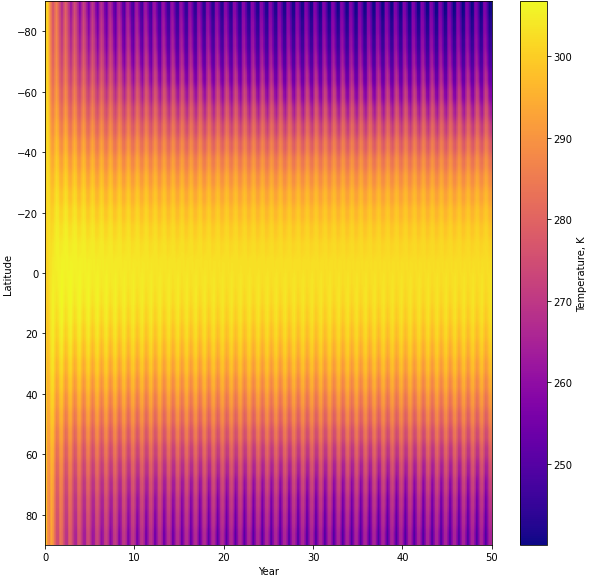
\includegraphics[width = 8cm]{Earth50yrsHeatmap.png}
  \caption{Heatmap of Earth climate between 0 - 50 years}
  \label{fig:sub1}
\end{subfigure}%
\begin{subfigure}{.5\textwidth}
  \centering
  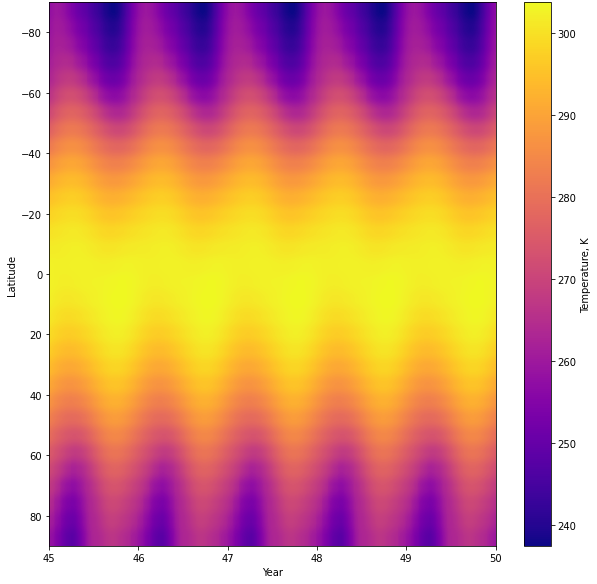
\includegraphics[width=8cm]{Earth5yrsHeatmap.png}
  \caption{Heatmap of Earth climate last 5 years of modelling}
  \label{fig:sub2}
\end{subfigure}
\raggedright
\caption{Heatmaps displaying Earth's climate (Kelvin) 50 years post model initialisation. Full heatmap (a) displays temperatures plotted every 73 days, settled heatmap (b) shows temperatures plotted every 5 days. Negative latitudes (degrees) correspond to the Southern hemisphere.}
\label{fig:test}
\end{figure}

The model solution under Earth parameters is compared to an empirical model formulated from observational data \cite{NC79},

\begin{center}
$T(x) = 302.3 - 45.3 \sin^{2}\lambda,$
\end{center}

where $x$ $\equiv \sin\lambda$. This fit does not account for asymmetric seasonal variations induced by the inclusion of Earths eccentricity, regardless, it describes the planets annual mean temperature per latitude well enough to assess the models' validity. A ten-year running annual mean is taken after every year of the models evolution past year 9. The mean relative difference across all latitudes is taken. Convergence is assessed by comparison to the above fit (X) every year, and also comparison to the models own temperatures at the same point in orbit each year. The convergence tests are found in Fig. (X).

\begin{figure}[t]
%\centering
\begin{subfigure}{.5\textwidth}
  \centering
  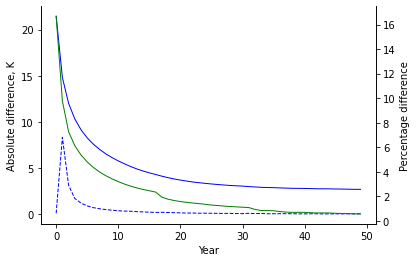
\includegraphics[width = 8cm]{Convergence.png}
  \caption{Earth convergence tests}
  \label{fig:sub1}
\end{subfigure}%
\begin{subfigure}{.5\textwidth}
  \centering
  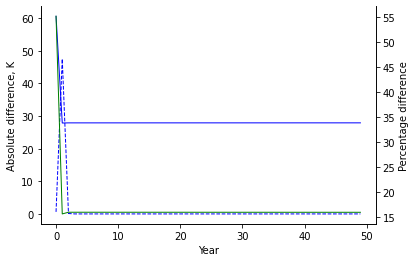
\includegraphics[width=8cm]{MarsConvergence.png}
  \caption{Mars convergence tests}
  \label{fig:sub2}
\end{subfigure}
\raggedright
\caption{Convergence tests for both planet models. Blue tests indicate comparison to empirical models (X), (X) by absolute (solid line) and percentage (dashed line) difference. Green test shows change in temperature compared to same time last year, $\delta$ = $|T_{year} - T_{year-1}|$. The average difference is taken at the Southern summer solstice.}
\label{fig:test}
\end{figure}

The Earth model settles to a less than 1\% difference to the empirical model.

\subsection{Mars}
Mars' model climate is compared to an analytical fit \cite{KH18} which is based on results from the NASA Ames GCM for a 7mbar atmosphere, 

\begin{center}
$T(x) = \frac{q_{0}}{4 \sqrt{1 - e^{2}}} \frac{S_{a_{0}}}{B} - \frac{A}{B} + \frac{q_{0}}{4 \sqrt{1 - e^{2}}} (\frac{S_{a_{2}}p_{2}(x)}{6D+B} + \frac{S_{a_{4}}p_{4}(x)}{20D+B})$,
\end{center}

where $q_{0}$ is the solar constant at Mars, $e$ is eccentricity, $D$ is diffusivity, and $x$ $\equiv \sin\lambda$ is the sine of the latitude. $A$, $B$, and $S_{a_{n}}$ are adjustable fitting parameters and $p_{n}$ are the Legendre polynomials.

\begin{figure}
%\centering
\begin{subfigure}{.5\textwidth}
  \centering
  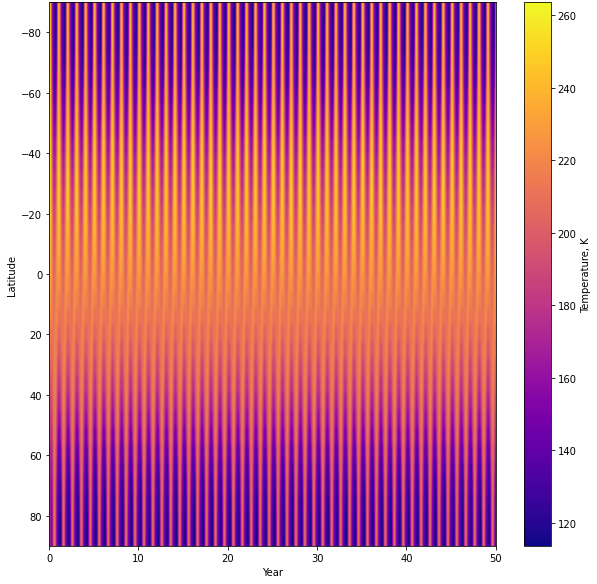
\includegraphics[width = 8cm]{Mars50yrsHeatmap.png}
  \caption{Heatmap of Mars climate between 0 - 50 years}
  \label{fig:sub1}
\end{subfigure}%
\begin{subfigure}{.5\textwidth}
  \centering
  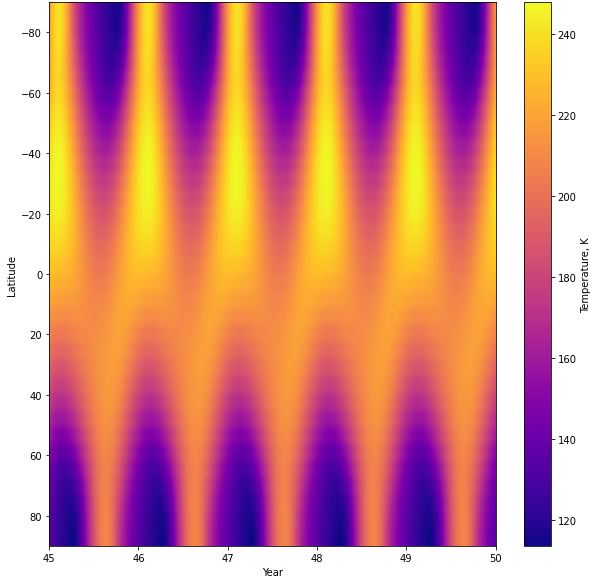
\includegraphics[width=8cm]{Mars5yrsHeatmap.png}
  \caption{Heatmap of Mars climate last 5 years of modelling}
  \label{fig:sub2}
\end{subfigure}
\raggedright
\caption{Heatmaps displaying Mars' climate (Kelvin) 50 years post model initialisation. Full heatmap (a) displays temperatures plotted every 3 days, as does settled heatmap (b). Negative latitudes (degrees) correspond to the Southern hemisphere.}
\label{fig:test}
\end{figure}

The model settles to a 16\% difference averaged over all latitudes to the model, although it is noted that this is taken as a latitudinal average on one day during the Southern summer and compared to annually averaged fit (X). Mean difference between the ten-year average and the analytical fit is 4.2K or 3.2\%.
Mars' heatmap displays much more relatively extreme summers and winters than Earth, as expected due to a much sparser atmosphere allowing for little heat diffusion (which is reflected in the diffusivity coefficient $D$ for each planet). The Southern hemisphere displays characteristically hot summers and cold winters relative to the milder North.

The assumption of equal land:ocean distribution in each latitude band is more justified in the case of Mars than Earth considering it is 100\% land, thus...


\section{Further Application to Mars}
\subsection{CO2 Cycle Modelling}

It will be assumed that the amount of CO2 adsorbed and released from the regolith annually is negligible, so that the total conserved amount of CO2 on Mars will always be split between ice on the ground and gaseous CO2 in the atmosphere. Previous EBMs have also excluded the contribution of the regolith and reached the same conclusions as models including it \cite{NT01}. %need something about how much is stored/released from regolith annually 
Further, it is assumed that the entire atmosphere of Mars is composed of CO2 [seasonal CO2 cycle James, North]
\begin{acknowledgments}
\end{acknowledgments}

%\bibliography{Draft1Notes}
\begin{thebibliography}{}

\bibitem{SMS08} D. Spiegel, K. Menou, C. Scharf., "Habitable Climates", The American Astronomical Society, vol. 681, 1609-1623 (2008).

\bibitem{WK97} D. Williams, J. Kasting., "Habitable Planets with High Obliquities", Icarus, vol. 129, 254-267 (1997).

\bibitem{AF89} J. Appelbaum, D. J. Flood., "Solar Radiation on Mars", Lewis Research Center, Cleveland, Ohio, Tech. Memorandum 102299, 1989.

\bibitem{NC79} G. R. North, J. A. Coakley., "Differences between Seasonal and Mean Annual Energy Balance Model Calculations of Climate and Climate Sensitivity", Journal of the Atmospheric Sciences, vol. 36, 1189-1204 (1979).

\bibitem{GQ01} P. R. Goode et al., "Earthshine Observations of the Earth's Reflectance", Geophysical Research Letters, vol. 28, 1671-1674 (2001).

\bibitem{PP12} D. K. Perovich, C. Polashenki., "Albedo evolution of seasonal Arctic sea ice", Geophysical Research Letters, vol. 39 (2012).

\bibitem{KH18} A. Kling, R. Haberle., "An analytical climate model to reproduce first order, yearly-averaged, climatology on early Mars: implications for the ancient lakes in the Gale crater", European Planetary Science Congress, vol. 12, 697 (2018).

\bibitem{FHT98} F. Forget, F. Hourdin, O. Talagrand., "CO2 Snowfall on Mars: Simulation with a General Circulation Model", Icarus, vol. 131, 302-316 (1998).

\bibitem{NT01} T. Nakamura, E. Tajika., "Stability and evolution of the climate system of Mars", Earth Planets Space, vol. 53, 851-859 (2001).

\bibitem{CBZH} P. Ceppi et al., "Cloud feedback mechanisms and their representation in global climate models", Wiley Interdisciplinary Reviews.

\bibitem{FP96} F. Forget, J. B. Pollack., "Thermal infrared observations of the condensing Martian polar caps: CO2 ice temperatures and radiative budget", Journal of Geophysical Research, vol. 101, 16865-16880 (1996).

\bibitem{L20} G. Lohmann, "Temperatures from energy balance models: the effective heat capacity matters", European Geosciences Union, vol. 11, 1195-1208 (2020).

\bibitem{W16} R. D. Wordsworth, "The Climate of Early Mars", Annual Review of Earth \& Planetary Sciences, vol. 44, 1-31 (2016).
\bibitem{1}
\bibitem{1}
\bibitem{1}

\end{thebibliography} 

\newpage
 
\clearpage

\end{document}
